\documentclass[a4paper, 11pt]{article}

\usepackage[margin=1in]{geometry}

\usepackage{hyperref}
\usepackage{graphicx}
\usepackage{graphics}
\usepackage{verbatim}
\usepackage{listings}
\usepackage{color}

\begin{document}

\title{BANO protocol notes}
\author{texane@gmail.com}
\date{}

\maketitle

%% \newpage
%% \tableofcontents
%% \addtocontents{toc}{\protect\setcounter{tocdepth}{1}}


\clearpage
\section{Overview}

\paragraph{}
The BANO protocol has been designed to implement a wireless network where a
resourceful device known as the \textit{base} interacts with smaller devices
known as the \textit{nodes}. The protocol especially targets domotics applications,
but is not limited to them.

\paragraph{}
In a typical architecture, the base centralizes node information. It reports
node information to the user, and schedules appropriate actions based on the
user configuration.

\paragraph{}
To ease understanding, this document focuses on the common case where base and
node roles are clearly distinct. However, there is no strong limitation that
prevents a node to act as a base, and a base to act as a node. Also, the protocol
does not limit the base count.

\paragraph{}
The BANO protocol relies on 2 messages used between bases and nodes for accessing
$(key,value)$ pairs:
\begin{itemize}
\item the \textit{SET} message is used to set a value given a specific key,
\item the \textit{GET} message is used to get a value given a specific key.
\end{itemize}

\begin{figure}[!h]
\begin{center}
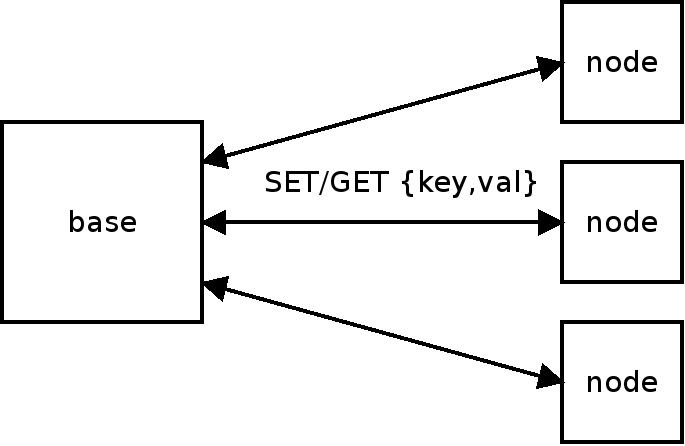
\includegraphics[scale=0.2]{../dia/overview_keyval/main.jpeg}
\end{center}
\caption{\tiny{key value exchange}}
\label{overview_keyval}
\end{figure}

\paragraph{}
These 2 messages are used to implement the following operations:
\begin{itemize}
\item \textit{synchronous SET} with optional acknowledgement: a base sets a
node value using a \textit{SET} message. If required, an acknowledgement can
be sent back as a flagged message,
\item \textit{synchronous GET}: a base gets a node value by sending a
\textit{GET} message, and waits for the corresponding reply,
\item \textit{asynchronous SET}: a base gets node key value pairs by listening
for incoming \textit{SET} messages.
\end{itemize}


%%
%% transport layer
\clearpage
\section{Transport layer}
\paragraph{}
BANO is designed for wireless networks. The hardware (RF chipsets) and logic
(low level protocol) used to transport messages are refer to as the
\textit{transport layer}. The following points were considered for choosing
a transport layer:
\begin{itemize}
\item packet based, with at least 16 bytes data payloads,
\item packet ordering is not required,
\item packet acknowledgement is not required,
\item packet routing is not required,
\item if provided by hardware, addressing must be at least 4 bytes. Otherwise,
addressing is implement in software and the payload size must be increased by 4
bytes,
\item if implemented by hardware, the CRC must be at least 2 bytes. Otherwise,
the CRC can be implemented in software.
\end{itemize}

\paragraph{}
After investigations, the following 2 chipsets from Nordic Semiconductor were
selected:
\begin{itemize}
\item NRF905 (covers sub GHz bands),
\item NRF24L01P (covers 2.4GHz band).
\end{itemize}


\clearpage
\section{Messages}

\subsection{Message format}

\paragraph{}
A message consists of a 128 bits sequence (16 bytes). Any field larger than 1
byte uses the little endian encoding. A header is always present and its format
is common to all the messages. The payload contents vary according to the operation.

\paragraph{}
\begin{figure}[!h]
\begin{center}
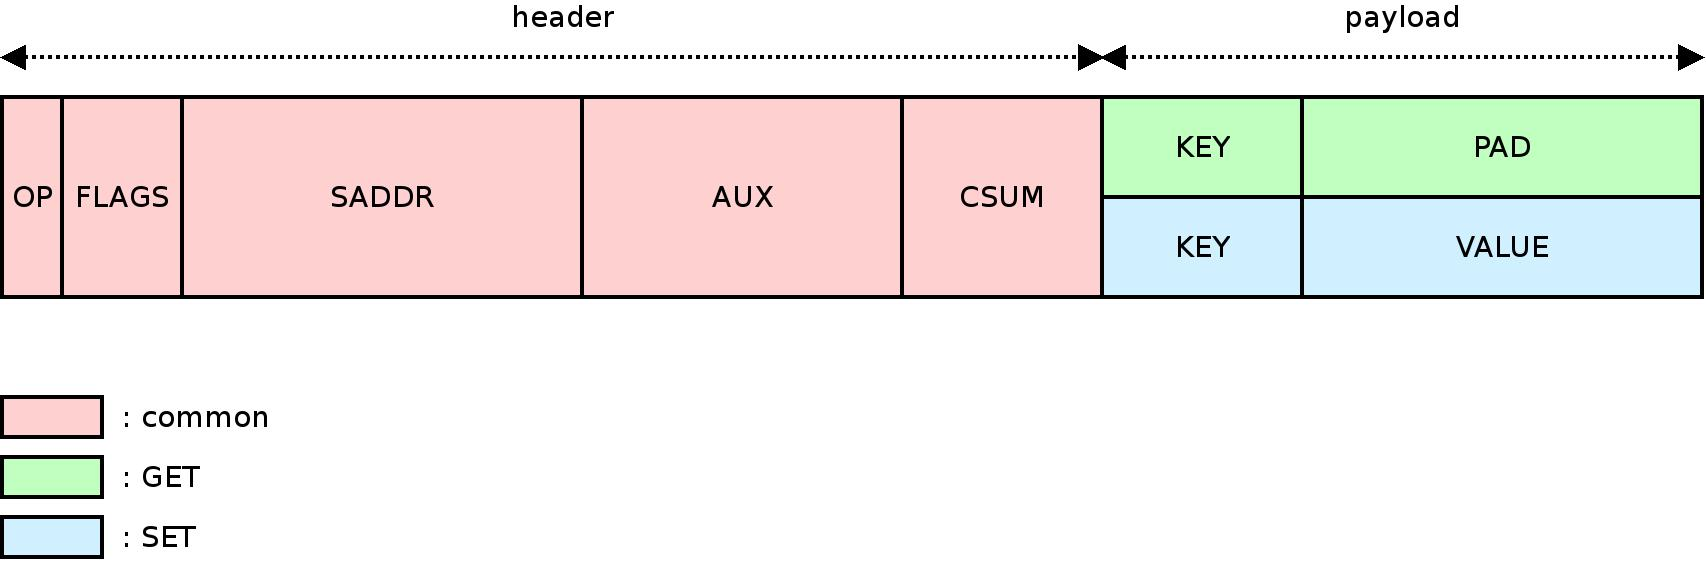
\includegraphics[scale=0.2]{../dia/msg_format/main.jpeg}
\end{center}
\caption{\tiny{message format}}
\label{msg_format}
\end{figure}

\begin{itemize}
\item \textit{OP}, 2 bits\\
One of the following message operation:
\begin{itemize}
\item BANO\_OP\_GET (0x0): get a value given a key,
\item BANO\_OP\_SET (0x1): set a value given a key.
\end{itemize}
\item \textit{FLAGS}, 6 bits\\
A combination of the following flags:
\begin{itemize}
\item BANO\_FLAG\_ACK ($1<<0$): this message acknowledges a previous one,
\item BANO\_FLAG\_REPLY ($1<<1$): this message replies a previous one,
\item BANO\_FLAG\_ERR ($1<<2$): error during operation execution.
\end{itemize}
\item \textit{SADDR}, 32 bits\\
The source address (sender node or base).
\item \textit{AUX}, 24 bits\\
Auxiliary data. Usage of this field is left to the application.
\item \textit{CSUM}, 16 bits\\
2 bytes checksum covering all the message bytes. During computation,
the CSUM field is considered zero. The use of a checksum is optional.
\item \textit{KEY}, 16 bits\\
The message target key.
\item \textit{VALUE}, 32 bits\\
The message target value. The protocol does not specify a format for
values. For instance, it can be used to transmit integer or real values.
\item \textit{PAD}, 32 bits\\
Padding. Contents are undefined.
\end{itemize}

\paragraph{}
NOTE: Currently, the destination address is handled by the transport layer,
and is not part of the message format. On the contrary, the source address
is not handled by the transport layer and is included in the message.

\paragraph{}
NOTE: if a checksum is already computed by the transport layer hardware, the
CSUM is not used.

\subsection{Message integrity}
\paragraph{}
\textbf{TODO}

\subsection{Message acknowledgement}
\paragraph{}
\textbf{TODO}

\subsection{Message forwarding}
\paragraph{}
\textbf{TODO} repeater


%%
%% addressing
\clearpage
\section{Addressing}

\paragraph{}
Bases and nodes are identified using 32 bits \textit{addresses}. Bases use a
known static address. Node addresses are randomly generated at programming time,
along with a random 32 bits \textit{seed}. If required, the following mechanism
is proposed to detect address collision.

\paragraph{} At any time, the base can detect by checking the uniqueness of
nodes $(addr,seed)$ pairs. To retrieve $(addr,seed)$ pairs, the base sends a
message to all the nodes that it has discovered so far:
%% msg.daddr = node_addr
%% msg.hdr.op = BANO_OP_GET
%% msg.hdr.flags = 0
%% msg.hdr.saddr = base_addr
%% msg.u.set.key = BANO_KEY_ADDR

\paragraph{}
Nodes reply with the following message:
%% msg.daddr = base_addr
%% msg.hdr.op = BANO_OP_SET
%% msg.hdr.flags = BANO_FLAG_REPLY
%% msg.hdr.saddr = node_addr
%% msg.u.set.key = BANO_KEY_ADDR
%% msg.u.set.val = node_seed

\paragraph{}
Address collision is detected if one or more identical $(addr,seed)$
pairs are received. The base resolves the conflict and sends new addresses
to the nodes:
%% msg.daddr = node_previous_addr
%% msg.hdr.op = BANO_OP_SET
%% msg.hdr.flags = 0
%% msg.hdr.saddr = node_new_addr
%% msg.u.set.key = BANO_KEY_ADDR
%% msg.u.set.val = node_seed


%%
%% security
\clearpage
\section{Security}

\paragraph{}
Implementing security adds complexity not required in all cases and goes
against some other BANO protocol design choices (stateless, common case,
short message size...). However, it is undeniable that there are node
messages that requiring some or all of the following security features:
\begin{itemize}
\item hiding message contents,
\item preventing replay attack,
\item preventing brute force,
\item preventing tampering attacks,
\item detecting node flood.
\end{itemize}

\paragraph{}
Each point is addressed in the following sections.

\subsection{Hiding message contents}
\paragraph{}
Symetric block ciphers can be used to hide message contents. The cipher
block size should comply with the BANO message size, ie. 16 bytes. Thus,
a 128 bits cipher is chosen (AES 128). Also, encryption is enabled for
all the messages of a given node. If this is a limitation, a node key
can allow the node to switch switch the encryption mode. In this case,
and because of statelessness, the encryption mode toggling should be
sent in 2 encrypted and clear versions.
\paragraph{}
Ciphers rely on a secret key shared between the base and the node. There
is no support for sharing the key built in the protocol. In a typical
situation, the node is programmed with a random key that is made known
to the base using the configuration interface.

\subsection{Preventing replay attack}
\paragraph{}
The usual way to prevent replay attack is for the node message to convey
a seed. This seed must not be known by the attacker at the time the message
is generated.
%% \paragraph{}
%% example: shutting down an alarm
%% An attacker may replay a previously capture message used to
%% unlock an alarm, even if encrypted. If the message contains
%% a time dependent information that can be checked by the base,
%% then any previously generated message will no longer be valid.
%% The time dependent information should be generated randomly
%% in a fashion not known by the attacker. For instance, a seed
%% can be generated locally by the base and sent encrypted to
%% the node.

\subsection{Preventing brute force}
\paragraph{}
\textbf{TODO}

\subsection{Preventing tampering attacks}
\paragraph{}
\textbf{TODO} man in the middle ...

\subsection{Detecting node flood}
\paragraph{}
\textbf{TODO}


%%
%% design considerations
\clearpage
\section{Design considerations}

\subsection{Focus on common case}
\paragraph{}
The protocol is designed with common case in mind. Any feature that is not
mandatory should not impact its design. For instance, security is a feature
that would impact message format if made mandatory. Another example is the
lack of message routing support.

\subsection{Node simplicity}
\paragraph{}
Nodes resource requirements should be as low as possible, enabling low cost
8 bits microcontroller based configurations. On the contrary, the base is
considered resourceful. This should be used to lower the node requirements.

\subsection{Low power consumption}
\paragraph{}
\textbf{TODO}
%% TODO: node mode (passive, listen only, time ...)

\subsection{Low memory footprint}
\paragraph{}
\textbf{TODO}

%% \subsection{Messaging}
%% \paragraph{}
%% in RX mode, a node receive logic consumes power. to reduce power consumption and
%% avoid being, a node can poll the requests by sending a request:
%% BANO_OP_GET, BANO_KEY_REQ, node_addr
%% the base must then send requests for this node in a short time lapse, and the
%% node will then return to reduced power mode at completion.
%% also, note the polling scheme prevents a malicious sender to
%% keep transmitting to a node in order to reduce its battery life.

%% TODO
%% [ on the assumption base is always present before nodes ]

%% A scenario where the user powers a node before powering the
%% base is largely possible. Handshaking .

%% Also, the base could be powered

%% Also, completely passive nodes (ie. alarm) does not anounce
%% themselves when powered up.

%% Thus, the base is not assumed to be present when a node is
%% added to the network.

%% (or base cannot assume base was present at the time
%% they do). Thus, there must be a mechanism to convey every
%% required information in one message.

%% Designing the protocol this way will increase


\end{document}
